\documentclass[aspectratio=169,10pt]{beamer}

\usepackage{fontspec}
\usepackage{array}
\usepackage{beamerthemeUQWeekly}

\defaultfontfeatures{Ligatures=TeX}
\setsansfont{Arial}[
  BoldFont=Arial Bold,
  ItalicFont=Arial Italic,
  BoldItalicFont=Arial Bold Italic
]
\setmainfont{Arial}[
  BoldFont=Arial Bold,
  ItalicFont=Arial Italic,
  BoldItalicFont=Arial Bold Italic
]
\newfontfamily\TitleSerif{Times New Roman}[
  BoldFont=Times New Roman Bold,
  ItalicFont=Times New Roman Italic,
  BoldItalicFont=Times New Roman Bold Italic
]
\renewcommand{\familydefault}{\sfdefault}

\hypersetup{
  unicode=true,
  pdftitle={Secure AI Workflow for Confidential Research},
  pdfauthor={},
  pdfsubject={Thesis weekly research progress},
  pdfkeywords={intranet AI, authorized retrieval, MCP, scientific software, secure release, blockchain},
  pdfcreator={XeLaTeX and Beamer}
}

\newcommand{\StudentName}{Chang Yin}
\newcommand{\SupervisorName}{Xiao Guo}
\newcommand{\PresentationDate}{5/8/2026}

\tikzset{
  workflowbox/.style={
    draw=black!35,
    fill=white,
    rounded corners=1.2pt,
    line width=0.55pt,
    minimum height=11mm,
    align=center,
    inner sep=1.2mm,
    font=\fontsize{8.0}{9.2}\selectfont
  },
  currentbox/.style={workflowbox,draw=StatusPinned,fill=StatusPinned!7},
  targetbox/.style={workflowbox,draw=StatusReview,fill=StatusReview!7},
  proposedbox/.style={workflowbox,draw=StatusLocal,fill=StatusLocal!8},
  neutralbox/.style={workflowbox,draw=black!35,fill=black!2},
  flowarrow/.style={draw=UQMuted,line width=0.9pt,-{Stealth[length=2mm]}},
  returnarrow/.style={draw=StatusReview,line width=0.85pt,-{Stealth[length=2mm]}},
  proofarrow/.style={draw=StatusLocal,line width=0.85pt,dashed,-{Stealth[length=2mm]}}
}

\begin{document}

% 1. Title
\begingroup
\UQUseTitleBackground
\begin{frame}[plain]
  \begin{tikzpicture}[remember picture,overlay]
    \node[
      anchor=north west,
      align=left,
      text width=118mm,
      inner sep=0pt,
      text=white
    ] at ([xshift=29.5mm,yshift=-16.2mm]current page.north west) {%
      {\TitleSerif\fontsize{20.0}{22.7}\selectfont Secure AI Workflow for\par Confidential Research}\par
      \vspace{2.5mm}
      {\fontsize{8.9}{10.8}\selectfont Authorized evidence, controlled tools, and accountable collaboration}
    };
    \node[
      anchor=north west,
      align=left,
      text width=98mm,
      inner sep=0pt,
      text=white
    ] at ([xshift=53.0mm,yshift=-43.8mm]current page.north west) {%
      \fontsize{9.9}{13.0}\selectfont
      \begin{tabular}{@{}>{\bfseries}l@{\hspace{3mm}}l@{}}
        Student: & \StudentName \\
        Supervisor: & \SupervisorName \\
        Date: & \PresentationDate
      \end{tabular}
    };
    \node[
      anchor=south east,
      align=right,
      text width=101mm,
      inner sep=0pt,
      text=white
    ] at ([xshift=-13.5mm,yshift=16.8mm]current page.south east) {%
      {\fontsize{10.6}{12.4}\selectfont School of Electrical Engineering and Computer Science}\par
      \vspace{1.1mm}
      {\fontsize{10.6}{12.4}\selectfont The University of Queensland}
    };
  \end{tikzpicture}
\end{frame}
\endgroup
\UQUseContentBackground

% 2. Research problem
\begin{frame}[plain,t]
\UQFrameHeader{Research Problem}{}{}
\begin{uqbody}
  \UQTakeaway{How can researchers use AI and scientific software without exposing confidential data?}

  \vspace{5.0mm}
  \begin{minipage}[t]{0.30\linewidth}
    {\color{StatusPinned}\rule{\linewidth}{1.2pt}}\par\vspace{1.8mm}
    {\fontsize{10.5}{12.2}\selectfont\bfseries Keep data inside}\par
    \vspace{2.4mm}
    Files and model context stay inside the protected network.
  \end{minipage}\hfill
  \begin{minipage}[t]{0.30\linewidth}
    {\color{StatusReview}\rule{\linewidth}{1.2pt}}\par\vspace{1.8mm}
    {\fontsize{10.5}{12.2}\selectfont\bfseries Use permitted evidence}\par
    \vspace{2.4mm}
    Only approved evidence reaches the model.
  \end{minipage}\hfill
  \begin{minipage}[t]{0.30\linewidth}
    {\color{StatusLocal}\rule{\linewidth}{1.2pt}}\par\vspace{1.8mm}
    {\fontsize{10.5}{12.2}\selectfont\bfseries Control every action}\par
    \vspace{2.4mm}
    Narrow interfaces control tools and release.
  \end{minipage}

  \vspace{7.0mm}
  \centering
  {\fontsize{11.0}{13.0}\selectfont\bfseries One researcher experience; several independent trust boundaries.}\par
\end{uqbody}
\end{frame}

% 3. Target workflow
\begin{frame}[plain,t]
\UQFrameHeader{Target Workflow}{}{}
\begin{uqbody}
  \UQTakeaway{MCP is the controlled bridge between local AI, approved scientific software exports, and controlled external release.}

  \vspace{1.6mm}
  \UQStatusBadge{StatusDesign}{TARGET DESIGN}

  \vspace{3.2mm}
  \centering
  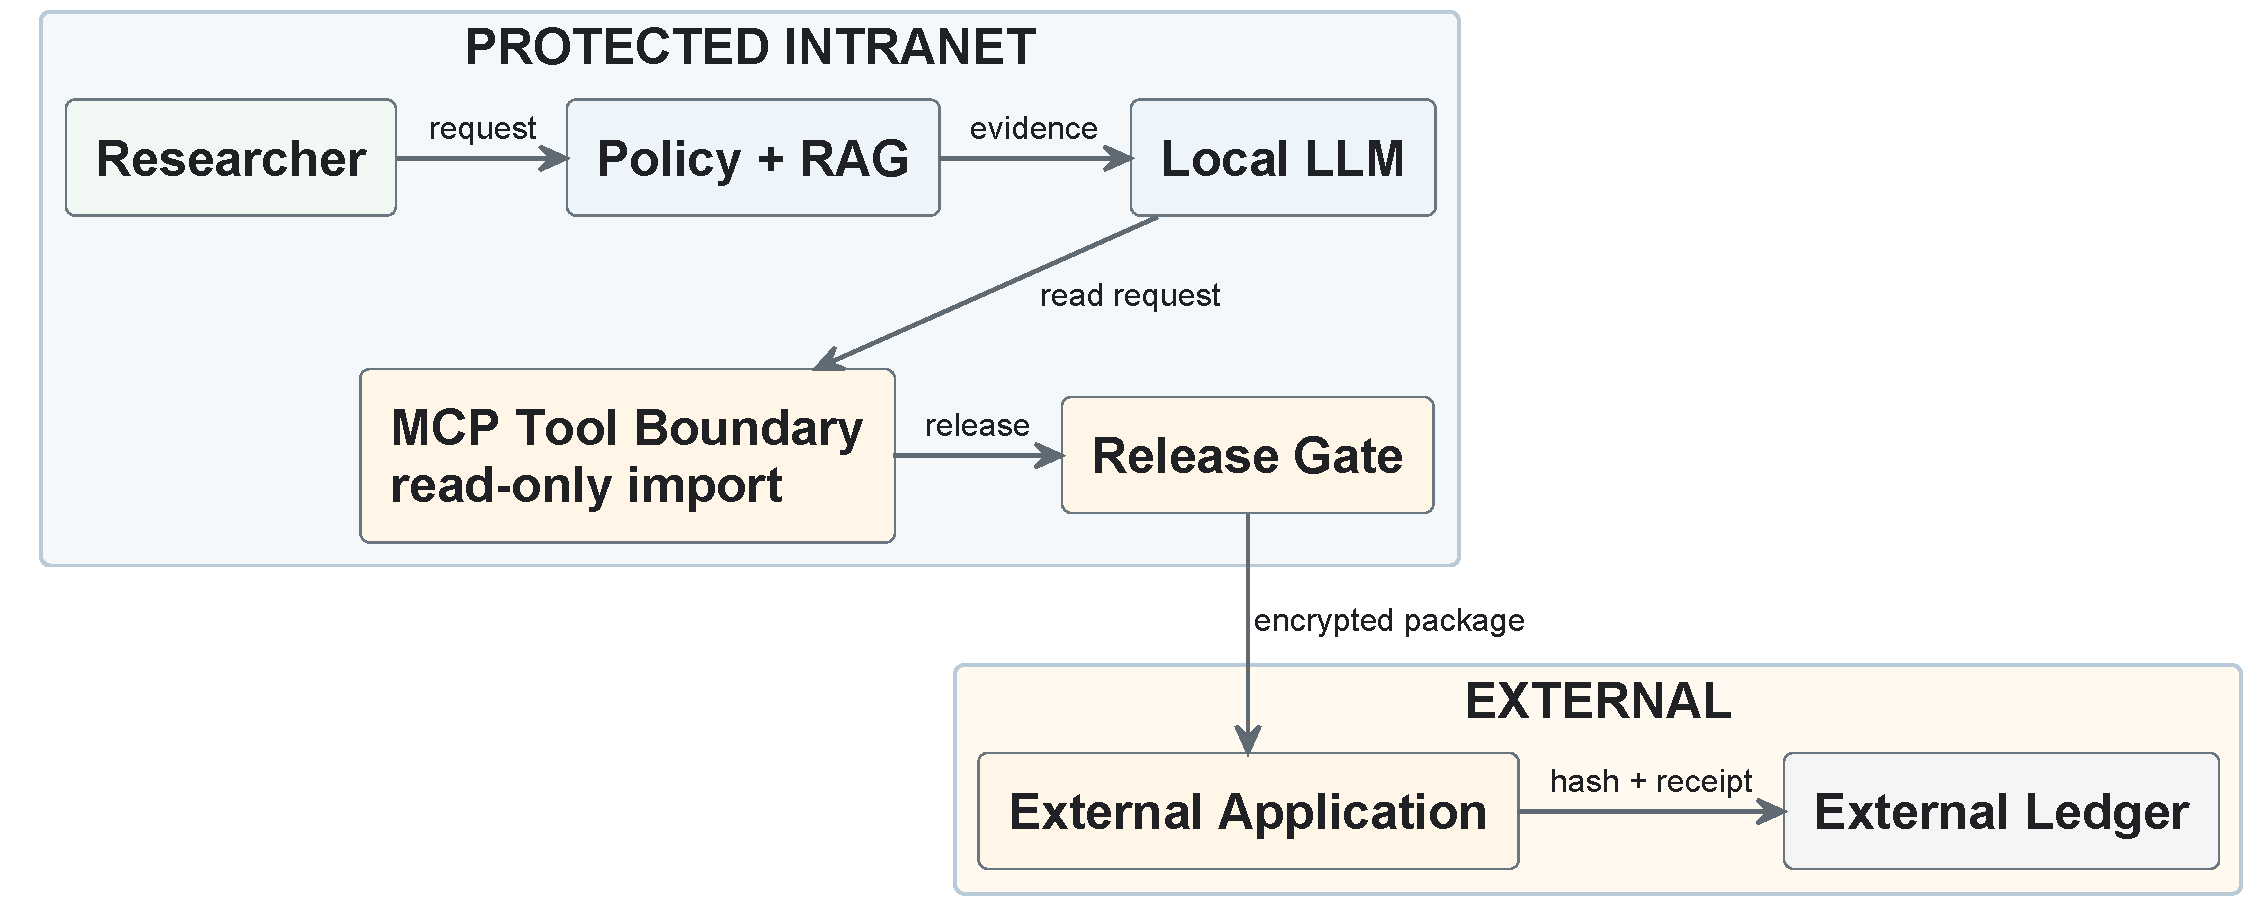
\includegraphics[width=\linewidth,height=38mm,keepaspectratio]{assets/diagrams/target-workflow.pdf}
\end{uqbody}
\end{frame}

% 4. Authorized retrieval
\begin{frame}[plain,t]
\UQFrameHeader{Authorize Before Retrieval}{}{}
\begin{uqbody}
  \UQTakeaway{An identity-aware agent gateway and policy authorize evidence before RAG; a separate model gateway invokes the registered local model.}

  \vspace{2.0mm}
  \UQStatusBadge{StatusDesign}{TARGET DESIGN}

  \vspace{4.0mm}
  \centering
  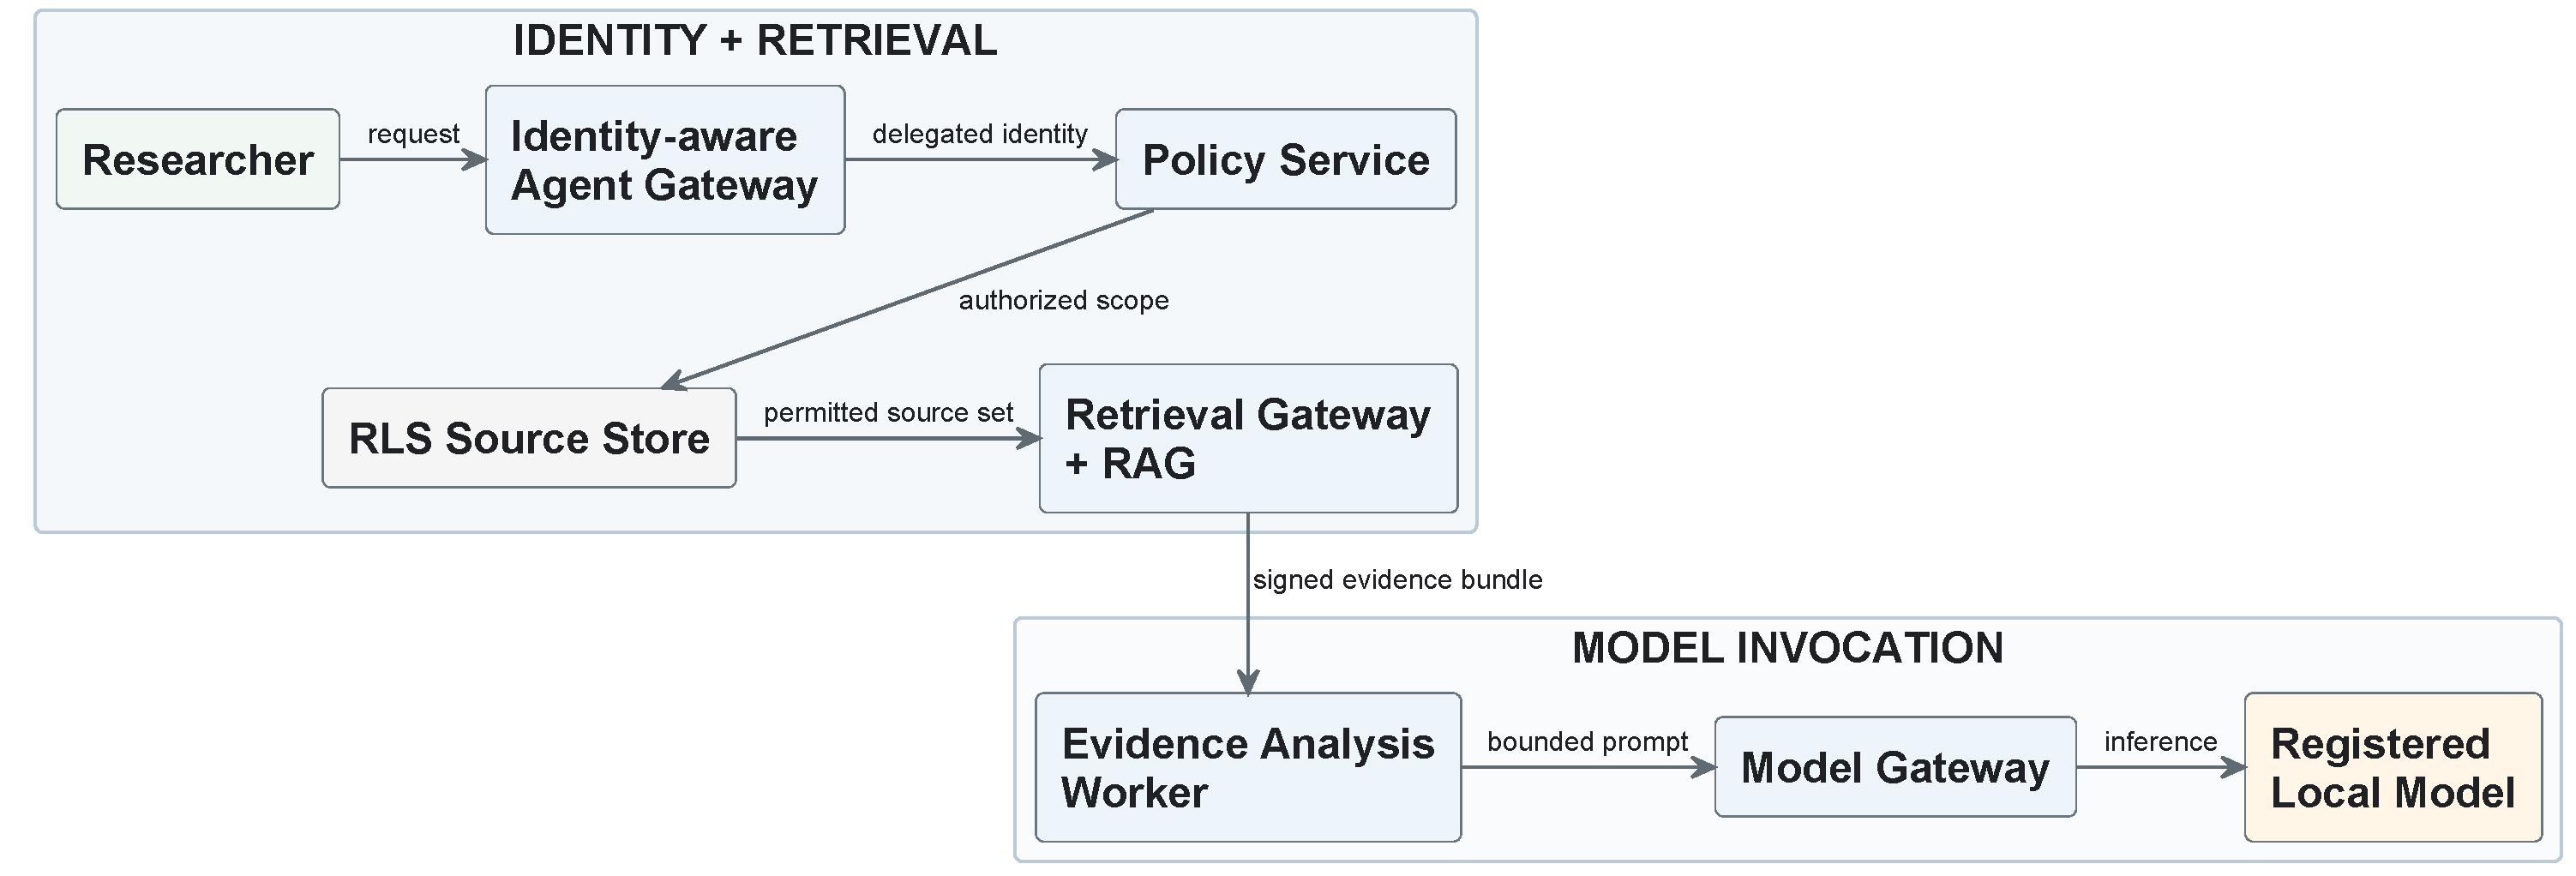
\includegraphics[width=\linewidth,height=38mm,keepaspectratio]{assets/diagrams/authorize-before-retrieval.pdf}
\end{uqbody}
\end{frame}

% 5. MCP and local scientific software
\begin{frame}[plain,t]
\UQFrameHeader{MCP as the Tool Boundary}{}{}
\begin{uqbody}
  \UQTakeaway{The model may request a bounded read-only import through a scientific software adapter; Tidy3D is the initial validation case.}

  \vspace{2.0mm}
  \UQStatusBadge{StatusLocal}{PROPOSED; INITIAL CASE: TIDY3D}

  \vspace{4.2mm}
  \centering
  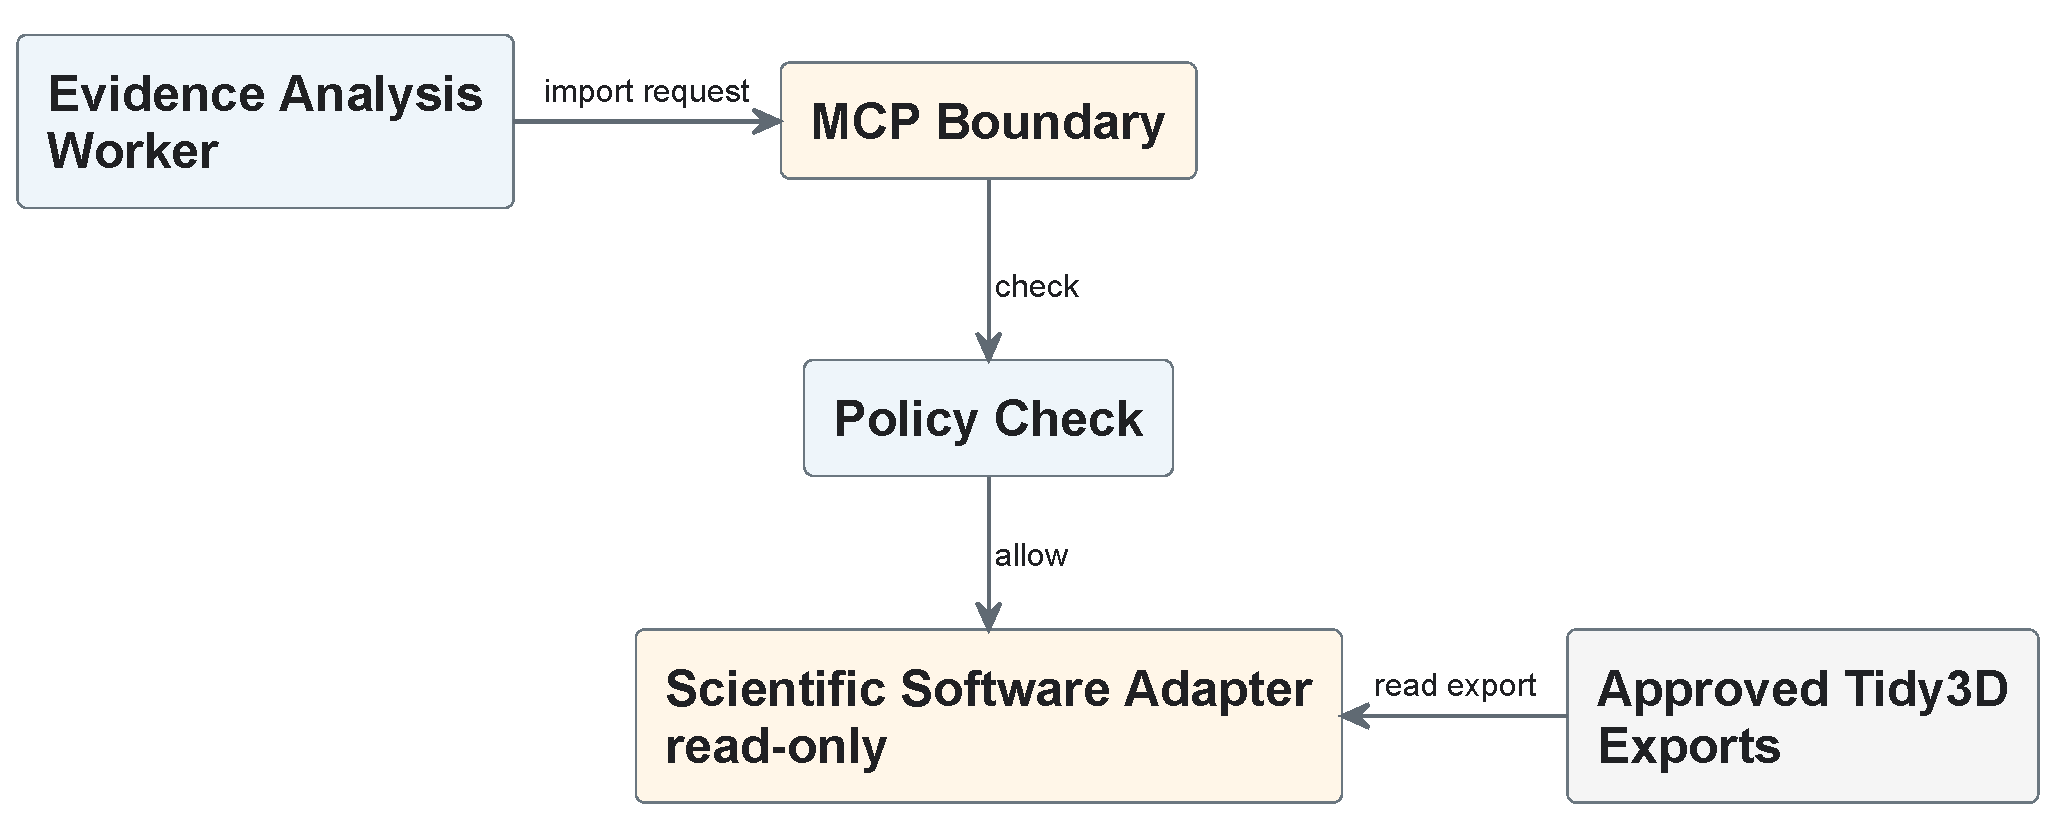
\includegraphics[width=\linewidth,height=38mm,keepaspectratio]{assets/diagrams/mcp-tool-boundary.pdf}

\end{uqbody}
\end{frame}

% 6. Secure collaboration and blockchain
\begin{frame}[plain,t]
\UQFrameHeader{Confidential Collaboration}{}{}
\begin{uqbody}
  \UQTakeaway{Confidential payloads stay in protected off-chain packages; the ledger stores only a minimal proof.}

  \vspace{2.0mm}
  \UQStatusBadge{StatusLocal}{CONCEPT; INTERFACE UNDEFINED}

  \vspace{4.0mm}
  \centering
  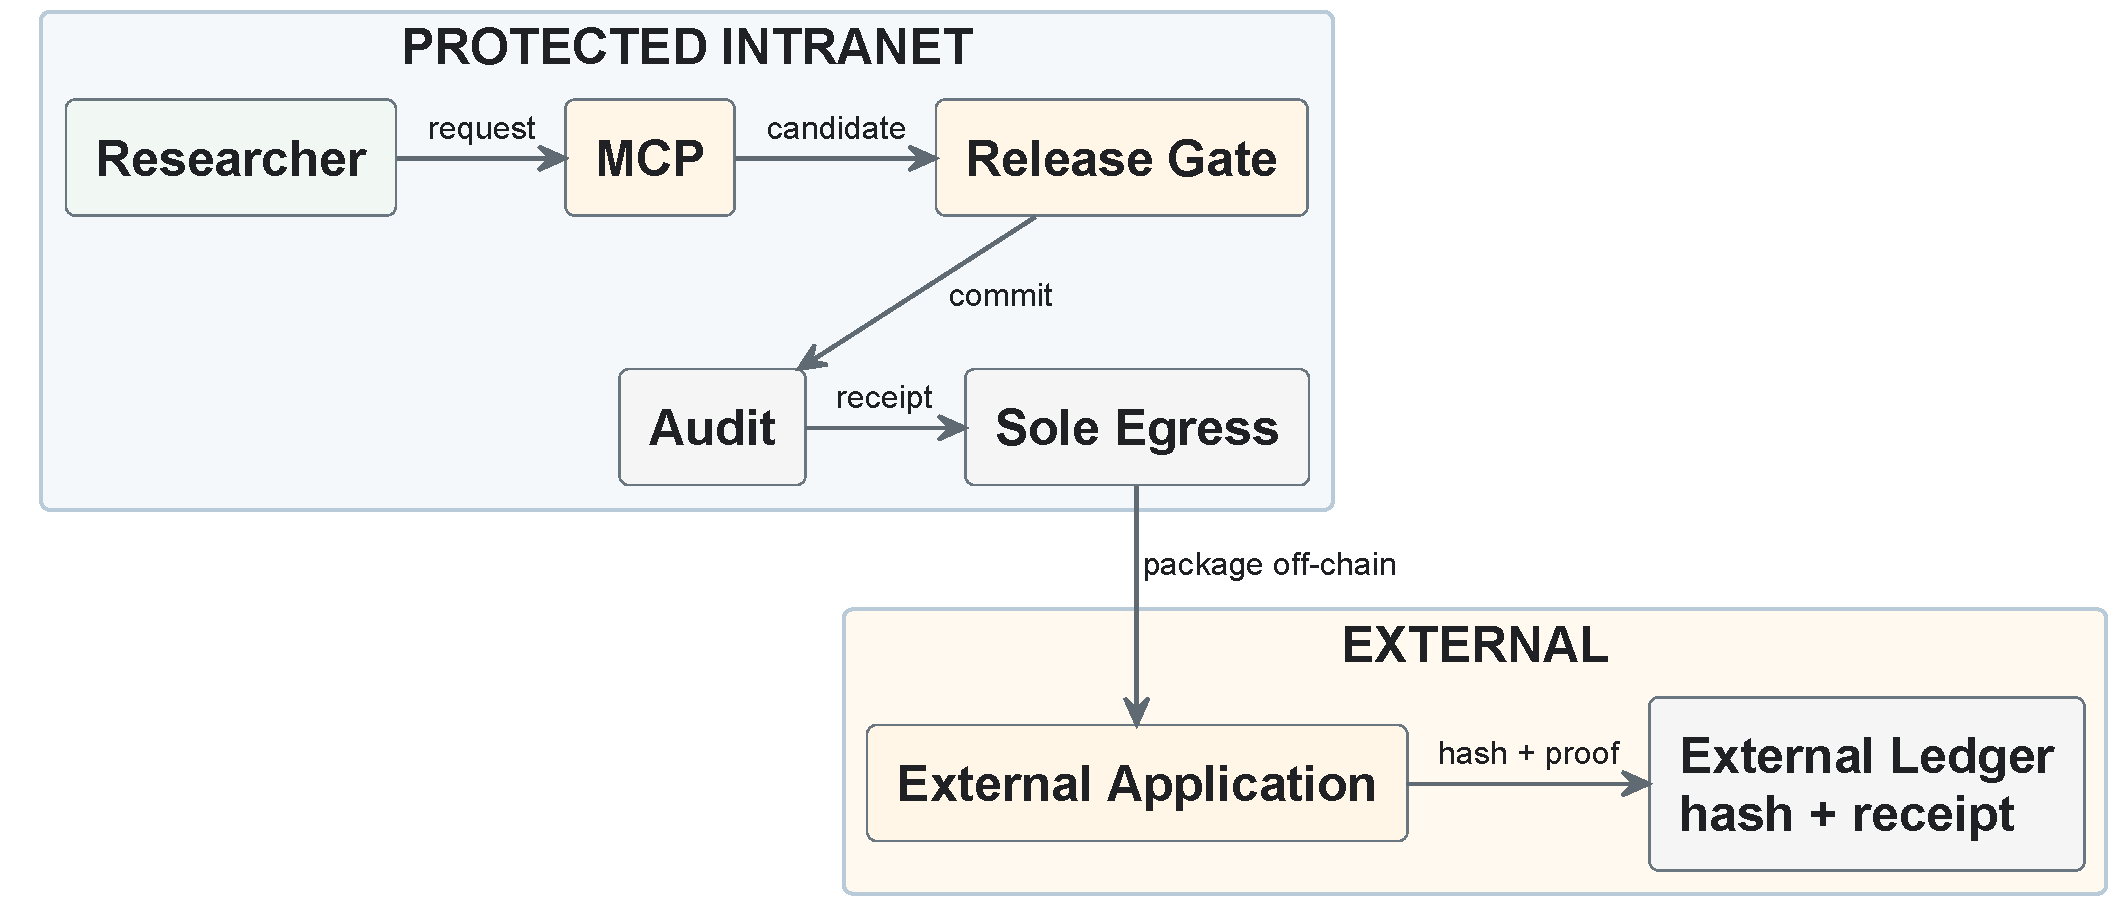
\includegraphics[width=\linewidth,height=38mm,keepaspectratio]{assets/diagrams/confidential-collaboration.pdf}

\end{uqbody}
\end{frame}

% 7. Model options
\begin{frame}[plain,t]
\UQFrameHeader{Model Options}{}{}
\begin{uqbody}
  \UQTakeaway{Model scale changes deployment; it does not replace authorization or review.}

  \vspace{1.7mm}
  \begin{minipage}[t]{0.48\linewidth}
    {\color{StatusReview}\rule{\linewidth}{1.2pt}}\par\vspace{0.8mm}
    {\color{StatusReview}\fontsize{6.8}{8.0}\selectfont\bfseries LOCAL-SCALE CANDIDATE}\par
    \vspace{0.7mm}
    \centering
    \begin{tikzpicture}[x=1cm,y=1cm]
      \clip (0,0) rectangle (6.45,2.10);
      \node[anchor=north west,inner sep=0pt] at (0,2.10) {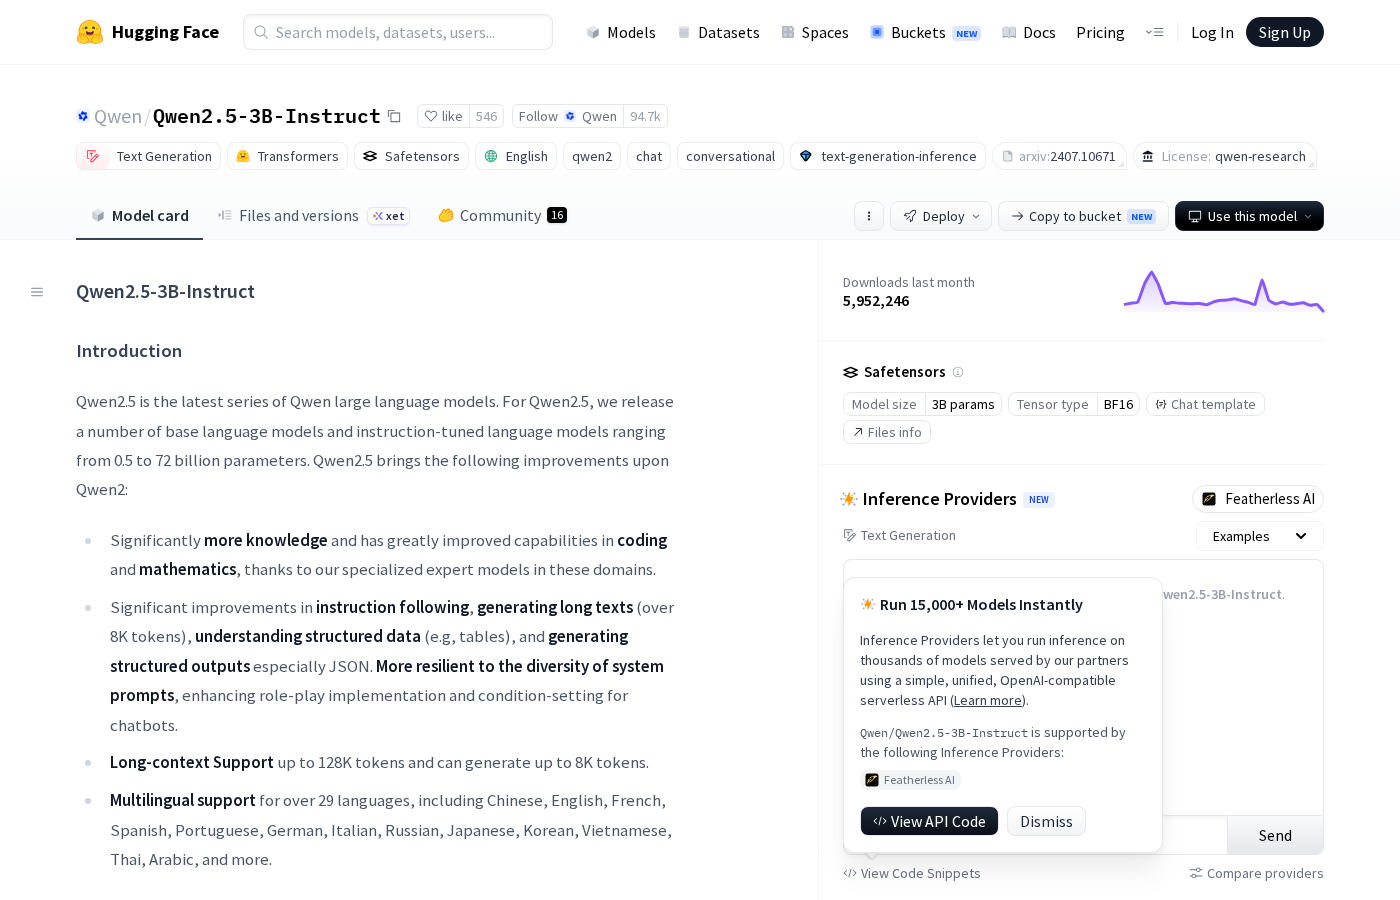
\includegraphics[width=84mm]{assets/qwen2.5-3b-model-page.png}};
      \draw[black!30,line width=0.45pt] (0,0) rectangle (6.45,2.10);
    \end{tikzpicture}\par
    \vspace{0.7mm}
    {\fontsize{9.4}{10.9}\selectfont\bfseries Qwen2.5-3B-Instruct}\par
    {\fontsize{8.0}{9.4}\selectfont 3B smoke-tested on one synthetic photonics fixture; not scientific validation.}\par
  \end{minipage}\hfill
  \begin{minipage}[t]{0.48\linewidth}
    {\color{StatusLocal}\rule{\linewidth}{1.2pt}}\par\vspace{0.8mm}
    {\color{StatusLocal}\fontsize{6.8}{8.0}\selectfont\bfseries CLUSTER-SCALE CANDIDATE}\par
    \vspace{0.7mm}
    \centering
    \begin{tikzpicture}[x=1cm,y=1cm]
      \clip (0,0) rectangle (6.45,2.10);
      \node[anchor=north west,inner sep=0pt] at (0,2.10) {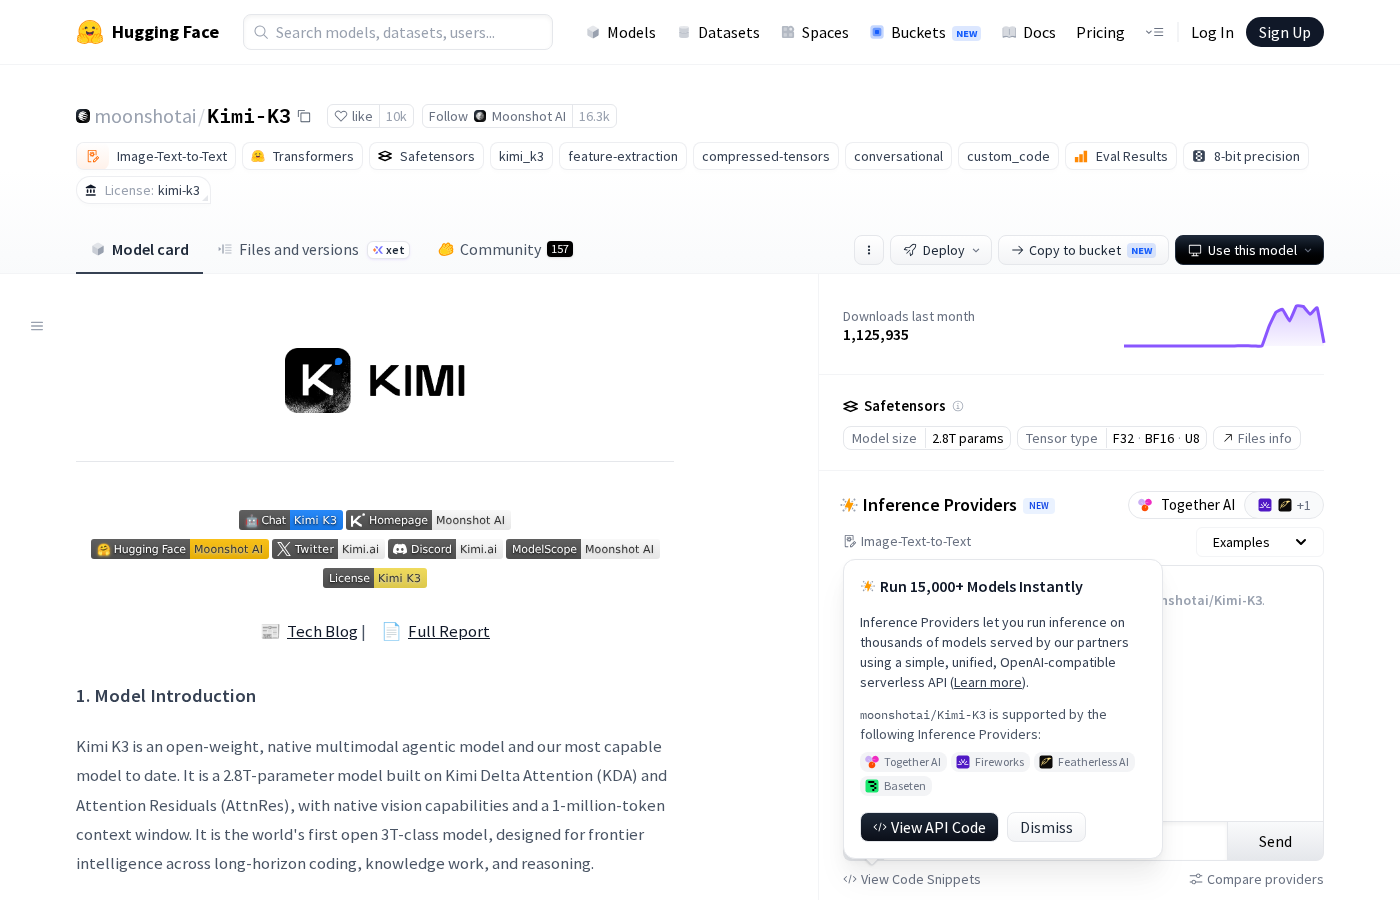
\includegraphics[width=84mm]{assets/kimi-k3-model-page.png}};
      \draw[black!30,line width=0.45pt] (0,0) rectangle (6.45,2.10);
    \end{tikzpicture}\par
    \vspace{0.7mm}
    {\fontsize{9.4}{10.9}\selectfont\bfseries Kimi K3}\par
    {\fontsize{8.0}{9.4}\selectfont Open-weight; 2.8T / 104B active; cluster-only.}\par
  \end{minipage}

  \vspace{1.4mm}
  \centering
  \UQStatusBadge{StatusPinned}{CURRENT EVIDENCE}\par
  \vspace{0.6mm}
  {\fontsize{8.6}{10.0}\selectfont\bfseries Current smoke test: qwen2.5:3b via loopback Ollama; qwen2.5:7b remains the handoff baseline. Neither candidate is enterprise integrated.}\par
\end{uqbody}
\end{frame}

% 8. Current evidence boundary
\begin{frame}[plain,t]
\UQFrameHeader{What Runs Today}{}{}
\begin{uqbody}
  \UQTakeaway{Only the local evidence workflow is operational; the intranet, MCP, and blockchain paths remain future work.}

  \vspace{3.0mm}
  \begin{tikzpicture}
    \fill[StatusPinned!7,rounded corners=1pt] (0,0) rectangle (13.75,1.25);
    \draw[StatusPinned!45,rounded corners=1pt,line width=0.55pt] (0,0) rectangle (13.75,1.25);
    \node[anchor=west,text=StatusPinned,font=\fontsize{7.2}{8.4}\selectfont\bfseries] at (0.35,0.92) {RUNS NOW};
    \node[anchor=west,text=UQInk,font=\fontsize{10.1}{11.8}\selectfont\bfseries] at (2.15,0.79) {Files $\rightarrow$ traceable evidence $\rightarrow$ local LLM $\rightarrow$ checked report};
    \node[anchor=west,text=UQInk,font=\fontsize{8.1}{9.5}\selectfont] at (2.15,0.32) {Single user, local access; public or synthetic data.};

    \fill[StatusReview!7,rounded corners=1pt] (0,-1.60) rectangle (13.75,-0.35);
    \draw[StatusReview!45,rounded corners=1pt,line width=0.55pt] (0,-1.60) rectangle (13.75,-0.35);
    \node[anchor=west,text=StatusReview,font=\fontsize{7.2}{8.4}\selectfont\bfseries] at (0.35,-0.68) {UNDER REVIEW};
    \node[anchor=west,text=UQInk,font=\fontsize{10.1}{11.8}\selectfont\bfseries] at (2.65,-0.98) {Stable interface between the agent and local model};

    \fill[black!3,rounded corners=1pt] (0,-3.20) rectangle (13.75,-1.95);
    \draw[black!25,rounded corners=1pt,line width=0.55pt] (0,-3.20) rectangle (13.75,-1.95);
    \node[anchor=west,text=StatusDesign,font=\fontsize{7.2}{8.4}\selectfont\bfseries] at (0.35,-2.28) {NOT BUILT};
    \node[anchor=west,text=UQInk,font=\fontsize{9.3}{10.7}\selectfont\bfseries] at (2.15,-2.58) {%
      \begin{tabular}{@{}l@{\hspace{3mm}\vrule\hspace{3mm}}l@{}}
        Authorized RAG & MCP tools\\
        Secure release & External ledger
      \end{tabular}%
    };
  \end{tikzpicture}
\end{uqbody}
\end{frame}

% 9. Engineering validation path
\begin{frame}[plain,t]
\UQFrameHeader{Engineering Validation Path}{}{}
\begin{uqbody}
  \UQTakeaway{Validate each trust boundary before connecting scientific tools or external networks.}

  \vspace{9.5mm}
  \centering
  \begin{tikzpicture}[
    stepbox/.style={
      draw=black!35,
      fill=white,
      rounded corners=1.2pt,
      line width=0.55pt,
      text width=22.2mm,
      minimum height=31mm,
      inner sep=1.5mm,
      align=left,
      font=\fontsize{7.7}{9.0}\selectfont
    },
    steparrow/.style={draw=UQMuted,line width=0.8pt,-{Stealth[length=1.8mm]}}
  ]
    \node[stepbox] (s1) {%
      \parbox[t][28mm][t]{22.2mm}{%
        \vspace{0pt}{\color{StatusReview}\fontsize{6.8}{8.0}\selectfont\bfseries 01 NOW}\par\vspace{1.2mm}
        {\fontsize{8.8}{10.2}\selectfont\bfseries Local model\\interface}\par\vspace{1.2mm}
        Finish review; record which model produced each output.%
      }%
    };
    \node[stepbox,right=2.7mm of s1] (s2) {%
      \parbox[t][28mm][t]{22.2mm}{%
        \vspace{0pt}{\color{StatusReview}\fontsize{6.8}{8.0}\selectfont\bfseries 02 NEXT}\par\vspace{1.2mm}
        {\fontsize{8.8}{10.2}\selectfont\bfseries Authorized\\retrieval}\par\vspace{1.2mm}
        Test access with\\synthetic data.%
      }%
    };
    \node[stepbox,right=2.7mm of s2] (s3) {%
      \parbox[t][28mm][t]{22.2mm}{%
        \vspace{0pt}{\color{StatusLocal}\fontsize{6.8}{8.0}\selectfont\bfseries 03 THEN}\par\vspace{1.2mm}
        {\fontsize{8.8}{10.2}\selectfont\bfseries Release\\protocol}\par\vspace{1.2mm}
        Define approval, encryption, and receipts.%
      }%
    };
    \node[stepbox,right=2.7mm of s3] (s4) {%
      \parbox[t][28mm][t]{22.2mm}{%
        \vspace{0pt}{\color{StatusDesign}\fontsize{6.8}{8.0}\selectfont\bfseries 04 GATED}\par\vspace{1.2mm}
        {\fontsize{8.8}{10.2}\selectfont\bfseries Science tool\\adapter}\par\vspace{1.2mm}
        Connect one read-only local adapter.%
      }%
    };
    \node[stepbox,right=2.7mm of s4] (s5) {%
      \parbox[t][28mm][t]{22.2mm}{%
        \vspace{0pt}{\color{StatusDesign}\fontsize{6.8}{8.0}\selectfont\bfseries 05 LAST}\par\vspace{1.2mm}
        {\fontsize{8.8}{10.2}\selectfont\bfseries Ledger\\checkpoint}\par\vspace{1.2mm}
        Use a ledger proof only if a real need remains.%
      }%
    };
    \draw[steparrow] (s1) -- (s2);
    \draw[steparrow] (s2) -- (s3);
    \draw[steparrow] (s3) -- (s4);
    \draw[steparrow] (s4) -- (s5);
  \end{tikzpicture}\par
\end{uqbody}
\end{frame}

% 10. Seven-day usage and cost
\begin{frame}[plain,t]
\UQFrameHeader{Seven-Day Usage and Cost}{}{}
\begin{uqbody}
  \UQTakeaway{01--07 Aug: usage is cache-heavy; a zero price estimate is not a zero operating cost.}

  \vspace{2.6mm}
  \begin{minipage}[t]{0.245\linewidth}
    {\color{StatusReview}\fontsize{6.8}{8.0}\selectfont\bfseries LOCAL CC-SWITCH}\par
    \vspace{1.2mm}
    {\color{StatusReview}\fontsize{16.5}{18.4}\selectfont\bfseries 4,635}\par
    {\fontsize{7.3}{8.6}\selectfont\bfseries requests}\par
    \vspace{1.8mm}
    {\color{StatusLocal}\fontsize{16.5}{18.4}\selectfont\bfseries 597M}\par
    {\fontsize{7.3}{8.6}\selectfont\bfseries total tokens}\par
    \vspace{1.8mm}
    {\color{StatusPinned}\fontsize{16.5}{18.4}\selectfont\bfseries 547M}\par
    {\fontsize{7.3}{8.6}\selectfont\bfseries cache reads}\par
    \vspace{1.8mm}
    {\color{StatusRisk}\fontsize{16.5}{18.4}\selectfont\bfseries \$0.00}\par
    {\fontsize{7.3}{8.6}\selectfont\bfseries interface estimate}\par
  \end{minipage}\hfill
  \begin{minipage}[t]{0.71\linewidth}
    {\fontsize{8.5}{10.0}\selectfont\bfseries Daily token trend from cc-switch}\par
    \vspace{1.3mm}
    \centering
    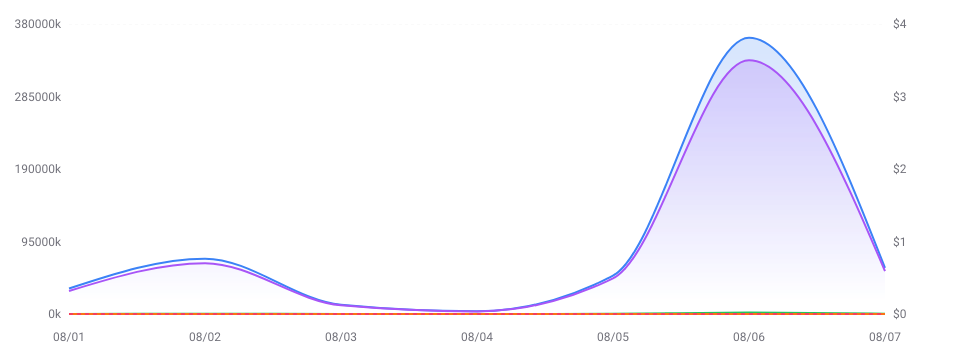
\includegraphics[width=\linewidth]{assets/cc-switch-usage-plot-7d-en.png}\par
    \vspace{0.8mm}
    {\fontsize{6.8}{8.0}\selectfont \textcolor{StatusReview}{Blue} = input tokens \quad
      \textcolor{purple}{purple} = cache reads \quad
      \textcolor{StatusRisk}{red} = estimated cost}\par
    \vspace{1.1mm}
    {\color{StatusRisk}\fontsize{7.1}{8.5}\selectfont\bfseries Cost interpretation:}\,
    {\fontsize{7.1}{8.5}\selectfont the \$0.00 interface estimate does not include hardware, cluster, or solver costs.}
  \end{minipage}
\end{uqbody}
\end{frame}

\end{document}
